At the end of Run 1, the LHC was shut down for upgrades and maintenance.
During this time, a number of upgrades were performed on the ATLAS detector, including the installation of a new innermost layer of the Pixel detector, the Insertable B-Layer (IBL)~\cite{2010.ibl-tdr}. \TODO{This will certainly be defined in the detector description, so maybe the citation and abbreviation are not needed}
These changes to the ID required some detector components to be removed temporarily, and many elements shifted relative to each other over the course of the maintenance process.
In order to correct for these large detector movements prior to \com{13} collision data taking, an alignment was performed using cosmic ray data collected in early 2015~\cite{2015.alignment-2015-cosmic}.
This alignment was able to correct for the majority of the large detector-wide misalignments as well as determine the global position of the IBL at the micron level.
%Due to the relatively low statistics available in the cosmic ray data, the alignment was performed up to L3 in the Pixel barrel and IBL and only up to L2 in the SCT (barrel and end-caps) and the Pixel end-caps; the TRT was kept fixed as a reference point.

In June of 2015, shortly after the data taking period began, the first track-based alignment of the refurbished ID was performed using $\mathcal{L} = 7.9~\mathrm{pb}^{-1}$ of \com{13} $pp$ collision data~\cite{2015.alignment-13tev}.
Starting from the initial geometry determined by the cosmic ray alignment, referred to hereafter as the \emph{March alignment}, an improved set of alignment constants, called the \emph{June alignment}, was derived from a data set of approximately 1.4 million selected tracks.
For comparison, a MC sample containing approximately 2.7 million tracks was constructed from dijet events simulated using a perfect detector geometry; the MC events are reweighted to match the $\eta$ and $\pt$ distributions found in the data.
Additional validation of the alignment results uses a set of cosmic ray data collected by the detector during the LHC collisions.
\TODO{find some way of saying that this section follows the alignment note~\cite{2015.alignment-13tev}? or is it ok not to...}

\subsection{June alignment procedure}
The data set used as the input for the alignment contains a subset of physics events used for prompt reconstruction recorded at a rate of 10~Hz.
To ensure that only high quality tracks are used for the alignment, each track is required to have transverse momentum $\pt > 3\gev$, contain at least one hit in the Pixel detector, at least seven hits in the combined silicon detectors, and at least 25 hits in the TRT.

A full L3 alignment of the IBL was included in the March alignment; however, the IBL was operated at a temperature of $-20^{\circ}\textrm{C}$ during the cosmic data taking and at $-10^{\circ}\textrm{C}$ for collision data taking.
This proved to be significant, as it was observed that the IBL staves experience a temperature-dependent parabolic bowing in the local $x'$-direction of approximately $-10\mum/\textrm{K}$~\cite{2015.alignment-ibl-stability}.
As a result, a new L3 alignment of the IBL was essential in order to correct for the bowing.
Due to it being a brand new element of the detector as well as its importance in vertexing and $b$ jet tagging, aligning the IBL sensors with a high degree of precision was of great importance.

The June alignment was performed in two stages.
The first pass focused on any relative movements of the big structures.
The March alignment corrected for these as well; however, it was observed during Run 1 that these sort of misalignments are introduced by changing conditions in the detector~\cite{2014.alignment-performance-8tev}, such as in the cooling system or magnet power cycling, which may have occurred between the early cosmic data taking and the first \com{13} collisions.
The TRT detector was kept fixed for the entire first pass to act as a global reference frame.
The full alignment chain for the first pass consisted of the following steps:
%\begin{table}[htbp]
%  \centering
%  \begin{tabular}{l | l | l}
%    Step & Subdetector & Specific alignment \\ 
%    \hline\hline
%    \multirow{5}{*}{1} & IBL & Aligned at L1 \\
%    \cline{2-3}
%                      & \multirow{2}{*}{Pixel} & Barrel aligned at L1 \\
%                      &                        & End-caps aligned at L1 \\
%    \cline{2-3}
%                      & \multirow{2}{*}{SCT} & Barrel and end-caps aligned at L1 (fixed in $T_z$)\\%\footnote{The SCT barrel is fixed in $T_z$ in order to constrain global displacements along the $z$-axis, since the TRT is not sensitive in this direction} \\
%                      &                      & End-caps aligned at L1 \\
%    \hline
%    \multirow{5}{*}{2} & IBL & Aligned at L2 \\
%    \cline{2-3}       & \multirow{2}{*}{Pixel} & Barrel aligned at L2 \\
%                      &                        & End-caps aligned at L2 \\
%    \cline{2-3}       & \multirow{2}{*}{SCT} & Barrel and end-caps aligned at L2 \\
%                      &                      & End-caps aligned at L1 \\
%    \hline
%    \multirow{5}{*}{3} & IBL & Aligned at L27 \\
%    \cline{2-3}       & \multirow{2}{*}{Pixel} & Barrel aligned at L27 \\
%                      &                        & End-caps aligned at L27 ($T_x$, $T_y$, and $R_z$ only) \\
%    \cline{2-3}       & \multirow{2}{*}{SCT} & Barrel and end-caps aligned at L2 \\
%                      &                      & End-caps aligned at L1 \\
%    \hline
%    4 & IBL & Aligned at L3 \\
%    \hline
%  \end{tabular}
%  \caption{}
%  \label{tab:align_2015_first_pass}
%\end{table}
\begin{enumerate}
\item The IBL, Pixel, and SCT detectors were aligned at L1.  The SCT barrel was not aligned in $T_z$ in order to constrain global displacements along the $z$-axis, as the TRT is not sensitive to that degree of freedom.
\item The IBL, and Pixel barrel and end-caps, and SCT barrel were aligned at L2.  The SCT end-caps were aligned at L1.
\item The IBL and pixel barrel were aligned at L27, using all six degrees of freedom.  The Pixel end-cap disks were only aligned in the plane ($T_x$, $T_y$, and $R_z$).  The SCT was treated the same as in the previous step.
\item The IBL was aligned at L3 using all six degrees of freedom for each module.
\end{enumerate}

The second pass was performed with the goal of improving the resolution on the transverse impact parameter of the tracks.
This step includes an added constraint, where an impact parameter with respect to the beam spot is added to the track as a pseudo-measurement.
When the alignment algorithm minimizes the $\chi^2$, it will take care of the impact parameter minimization as well.
Once again, the TRT was kept fixed.
The stages of the second pass are listed below:
\begin{enumerate}
\item The IBL and Pixel detectors were aligned at L2 with the SCT fixed.
\item The IBL was aligned at L27
\item The IBL and Pixel barrel and end-caps were aligned at L3.
\end{enumerate}
The set of alignment constants obtained at the end of the second pass represents the June alignment.
The highest level of alignment over the course of the two passes for each subdetector is listed in Table~\ref{tab:align_june_levels}.

\begin{table}[htbp]
  \centering
  \begin{tabular}{l l | l}
    Detector & & Highest level of alignment\\
    \hline\hline
    IBL && L3 \\
    \hline
    \multirow{2}{*}{Pixel} & Barrel & L3 \\
                           & End-caps & L3 ($T_x$, $T_y$, and $R_z$ only) \\
    \hline
    \multirow{2}{*}{SCT} & Barrel & L2 (except $T_z$) \\
                           & End-caps & L1 \\
    \hline
    TRT && None\\
    \hline
  \end{tabular}
  \caption{Summary of the highest level of alignment applied to each ID subsystem when deriving the June alignment.}
  \label{tab:align_june_levels}
\end{table}

\subsection{Alignment results}
The primary measure of alignment quality is assessed by looking at the track-hit residual distributions.
A well-aligned subdetector will have gaussian-distributed residuals centered at zero with a width approximating the detector's resolution.
The residual distributions are constructed from the same selection of tracks that were used to perform the alignment, and are the focus of Section~\ref{align:2015_results_residual}.
A second check on the alignment involves observables sensitive to the track parameter resolution.
In this case, cosmic rays are used, making use of a ``split track'' technique that takes advantage of the top-to-bottom cosmic ray trajectory (compared to the center-out trajectory of collision tracks).
These checks are detailed in Section~\ref{align:2015_results_cosmic}

\subsubsection{Residual distributions from collisions}\label{align:2015_results_residual}
As mentioned previously, the primary focus of the June alignment campaign was on the IBL and the Pixel detectors.
The detectors are the closest to the beam line and have the finest resolutions of the ID subdetectors.
The residual distributions in local $x$ and $y$ of the IBL planar sensors\footnote{The IBL contains 12 planar sensors in the center of a stave, with four 3D sensors on either end.  Only the planar sensors are shown here due to low statistics in the 3D sensors as well as poor MC modeling of these sensors.} are shown in Figure~\ref{fig:align_2015_results_ibl}.
These and subsequent figures in this section compare the June and March alignments to the perfectly-aligned MC simulation.
Noticeable improvement in the distribution widths can be seen in both the local $x$- and $y$-directions, nearly matching the simulation in local $x$, which is the most sensitive direction.

Due to the temperature-dependent bowing of the IBL, it is also interesting to look at the means of the residual distributions for each ring of IBL sensors along the beam line, as shown in Figure~\ref{fig:align_2015_results_ibl_z}.
A deformation is clearly visible in the March alignment in both measurement directions, and the shape in the local $x$-direction is consistent with an average stave bowing due to the different operating temperature of the IBL during the March alignment and the $13\tev$ collisions.
This feature was nearly eliminated in both directions through the L3 alignment of the IBL sensors.

The local $x$ and $y$ residual distributions for the Pixel detector barrel and end-caps are shown in Figure~\ref{fig:align_2015_results_pix}.
The IBL is not included in the plots of the barrel.
Once again, the June alignment outperforms the March alignment and rivals the simulation in all but the barrel local $y$ residuals, likely indicating that further refinement in the local $y$ alignment of the IBL was needed.

\begin{figure}[htbp]
  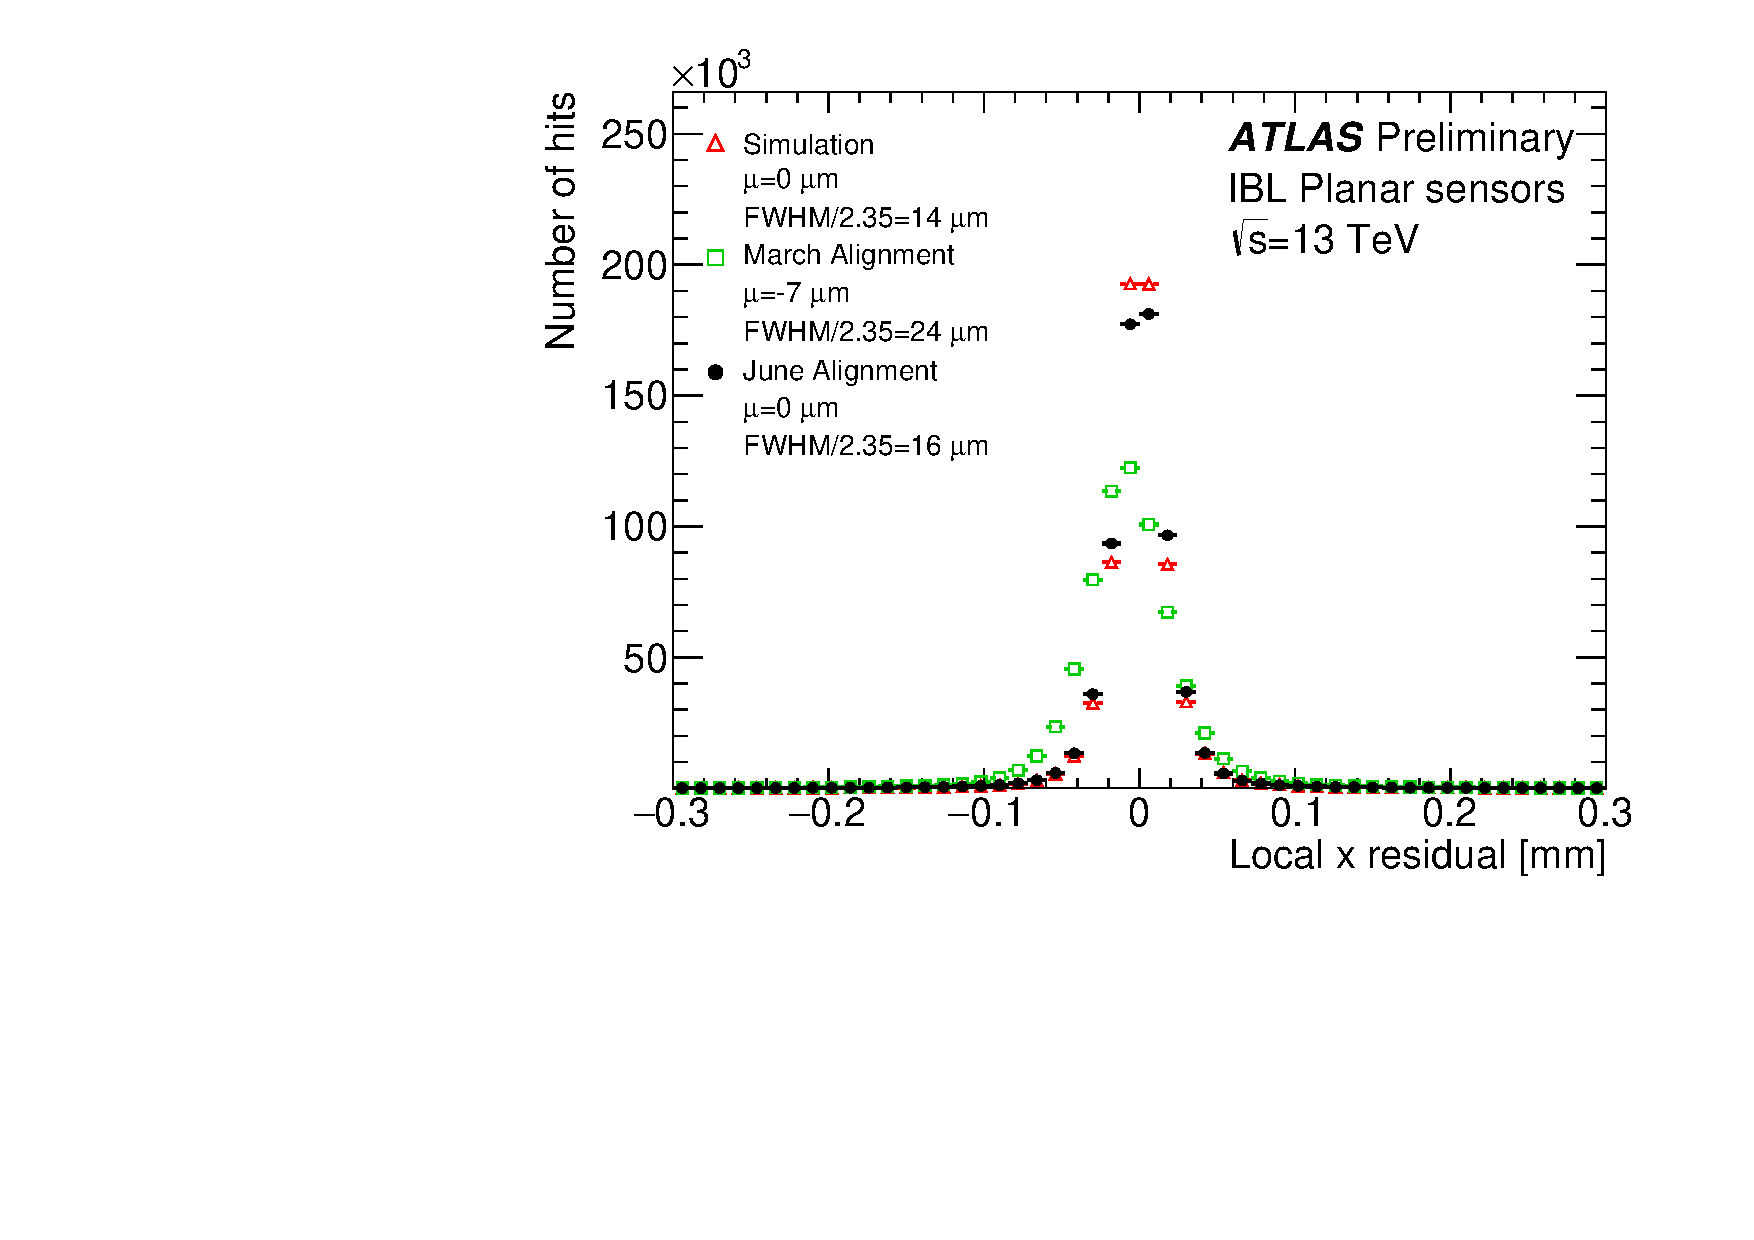
\includegraphics[width=.48\textwidth]{figs/alignment/align2015/PIXIBL_Planar_xRES}
  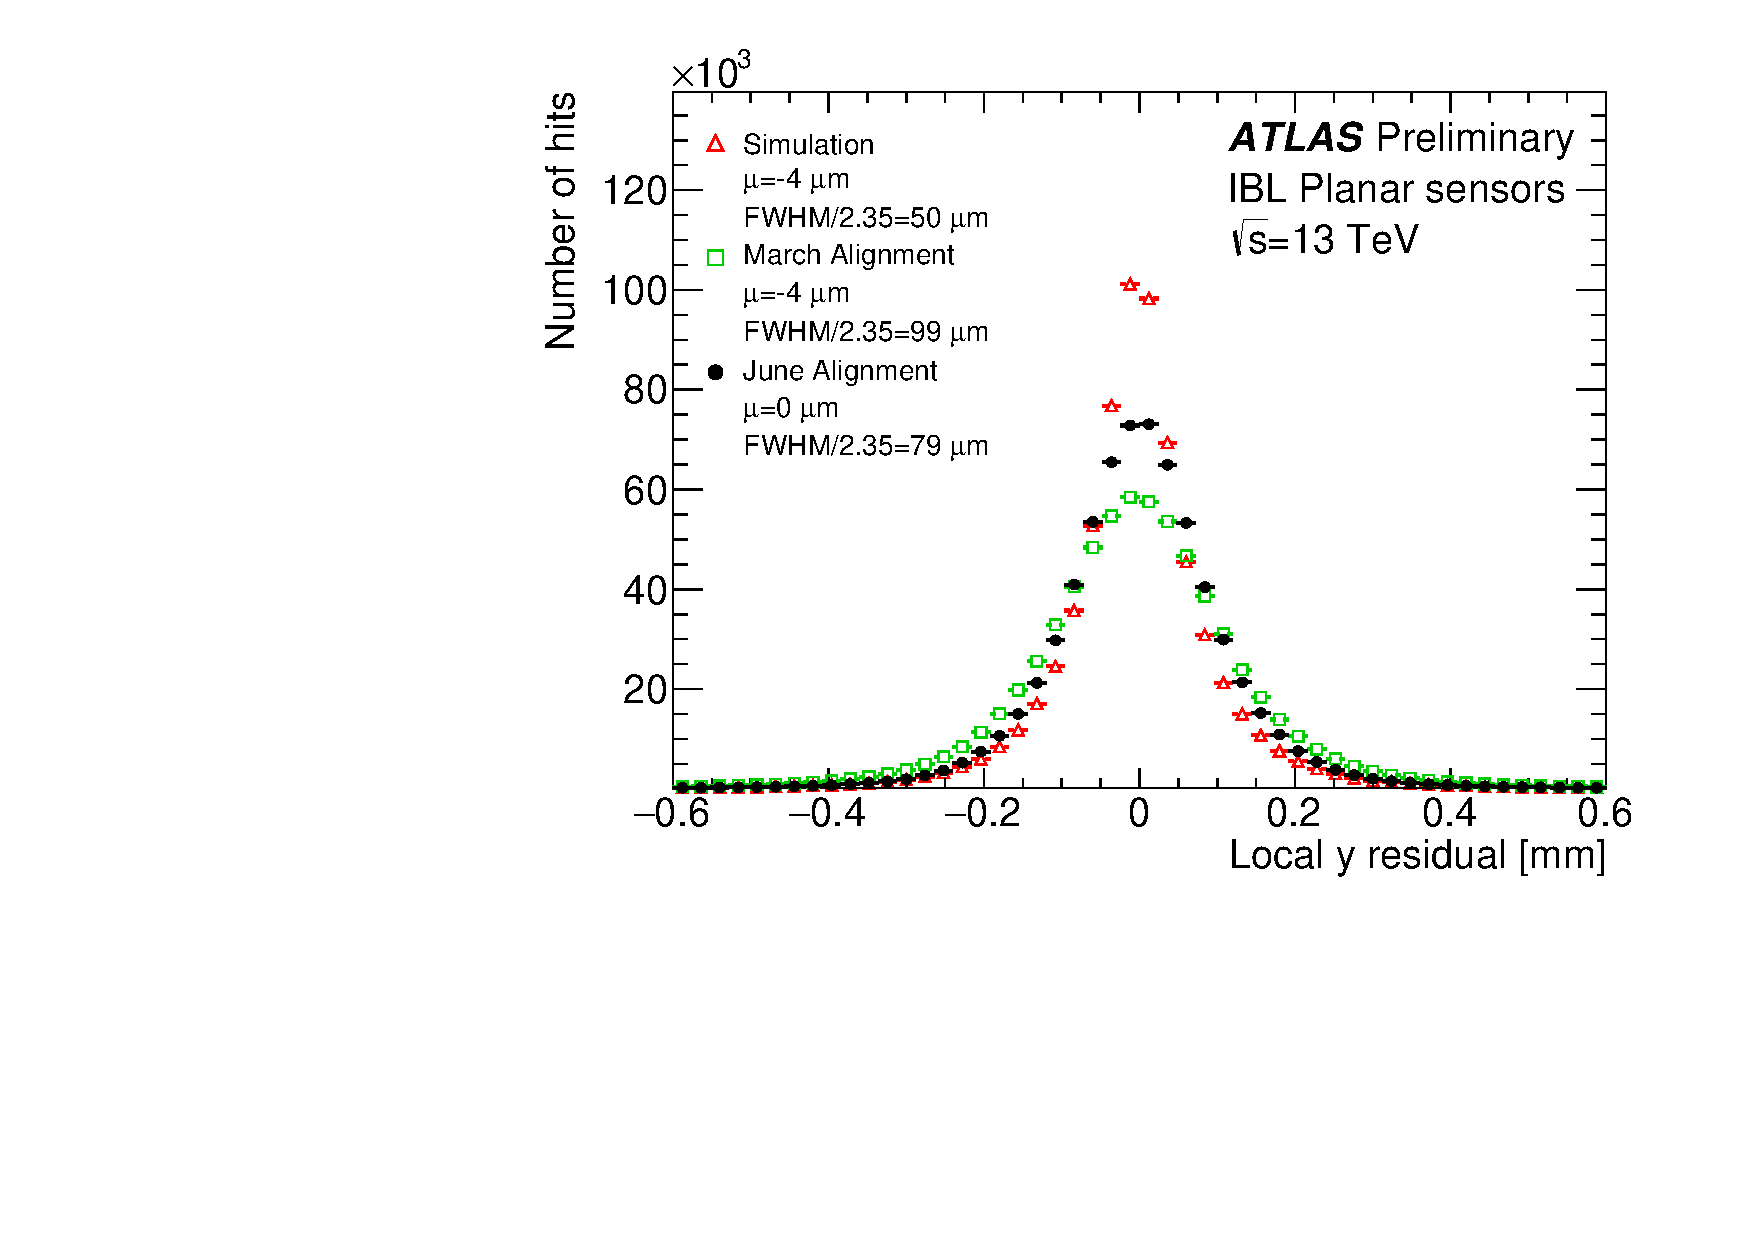
\includegraphics[width=.48\textwidth]{figs/alignment/align2015/PIXIBL_Planar_yRES}
  \caption{Local $x$ (left) and local $y$ (right) residual distributions of the IBL planar sensors using the \com{13} collision data sample reconstructed using the June (black) and March (green) alignments.  The data is compared to a MC simulation using a perfect detector geometry (red).  The distributions are normalized to the same number of entries.}
  \label{fig:align_2015_results_ibl}.
\end{figure}

\begin{figure}[htbp]
  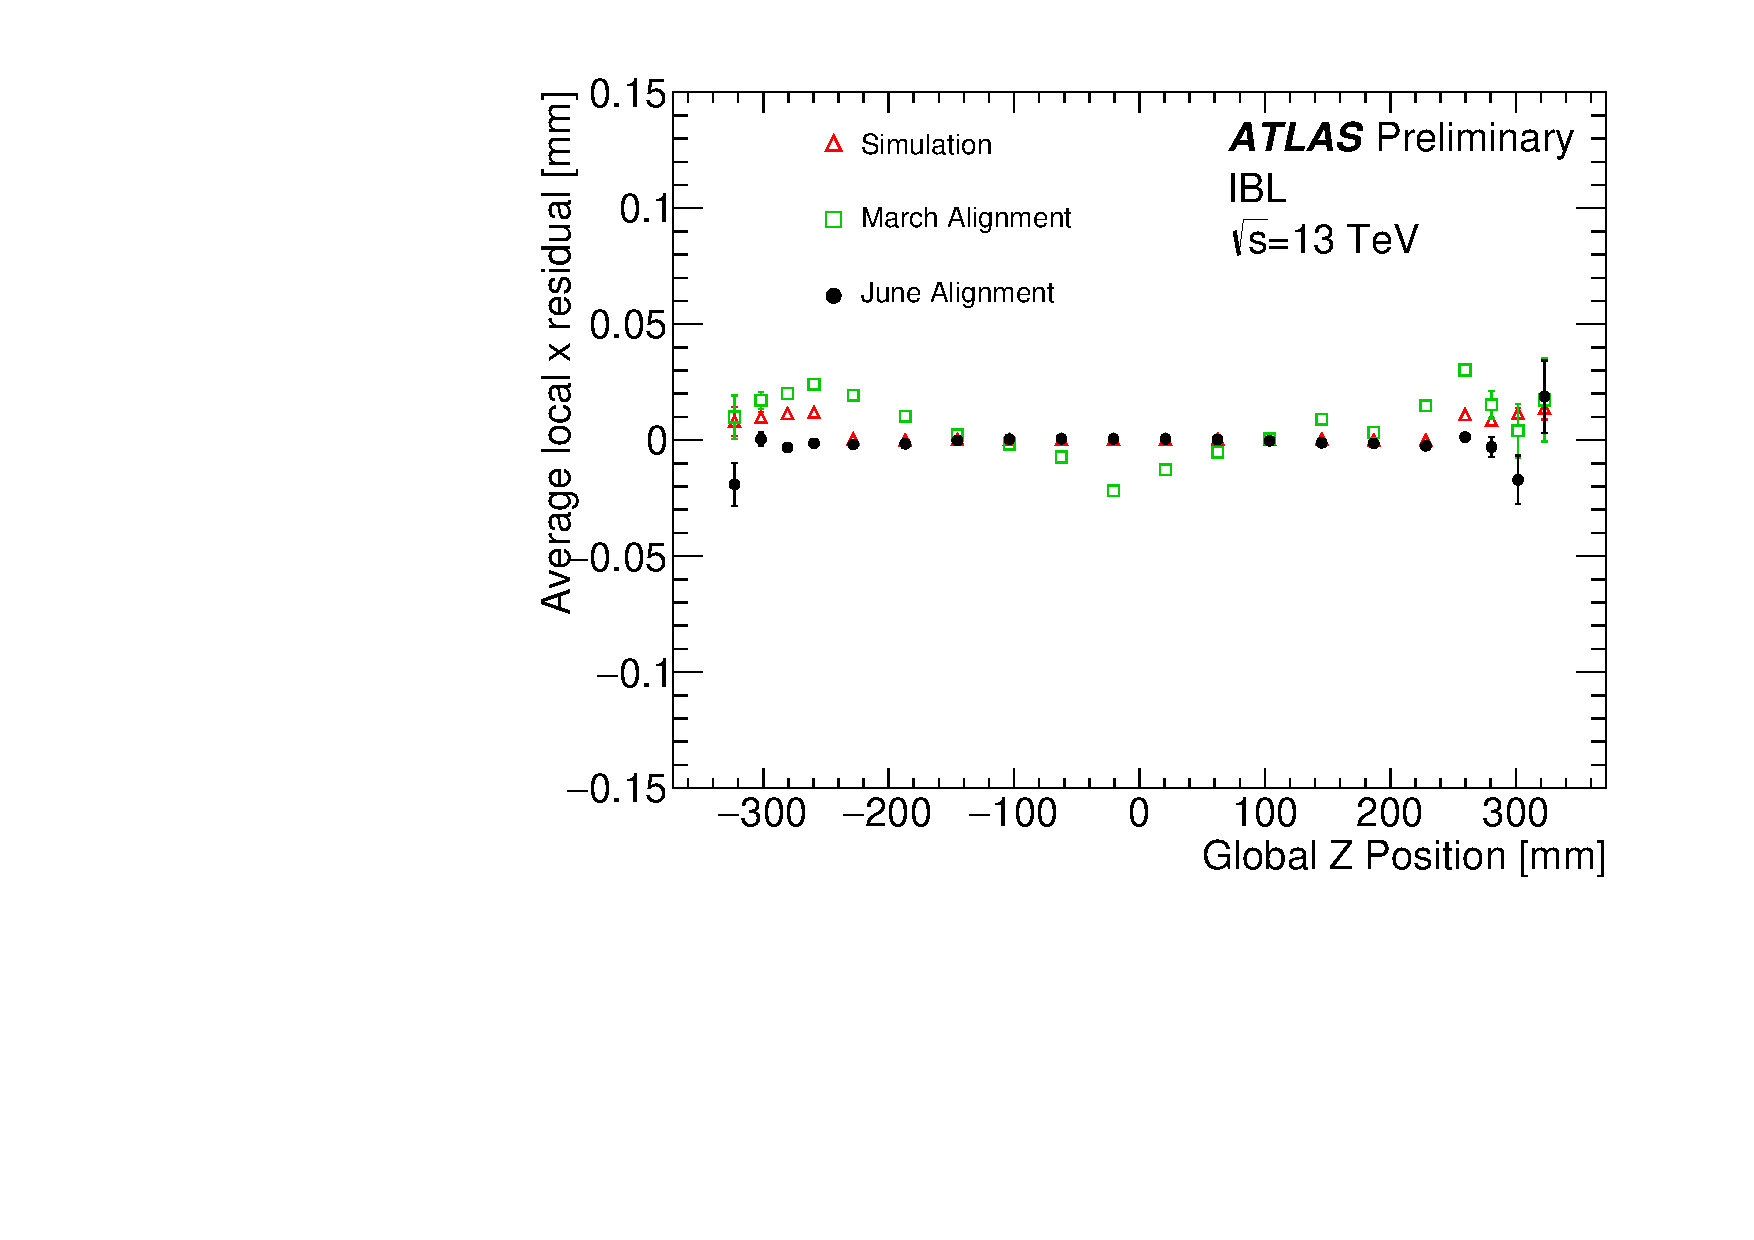
\includegraphics[width=.48\textwidth]{figs/alignment/align2015/IBL_xRESvsZ}
  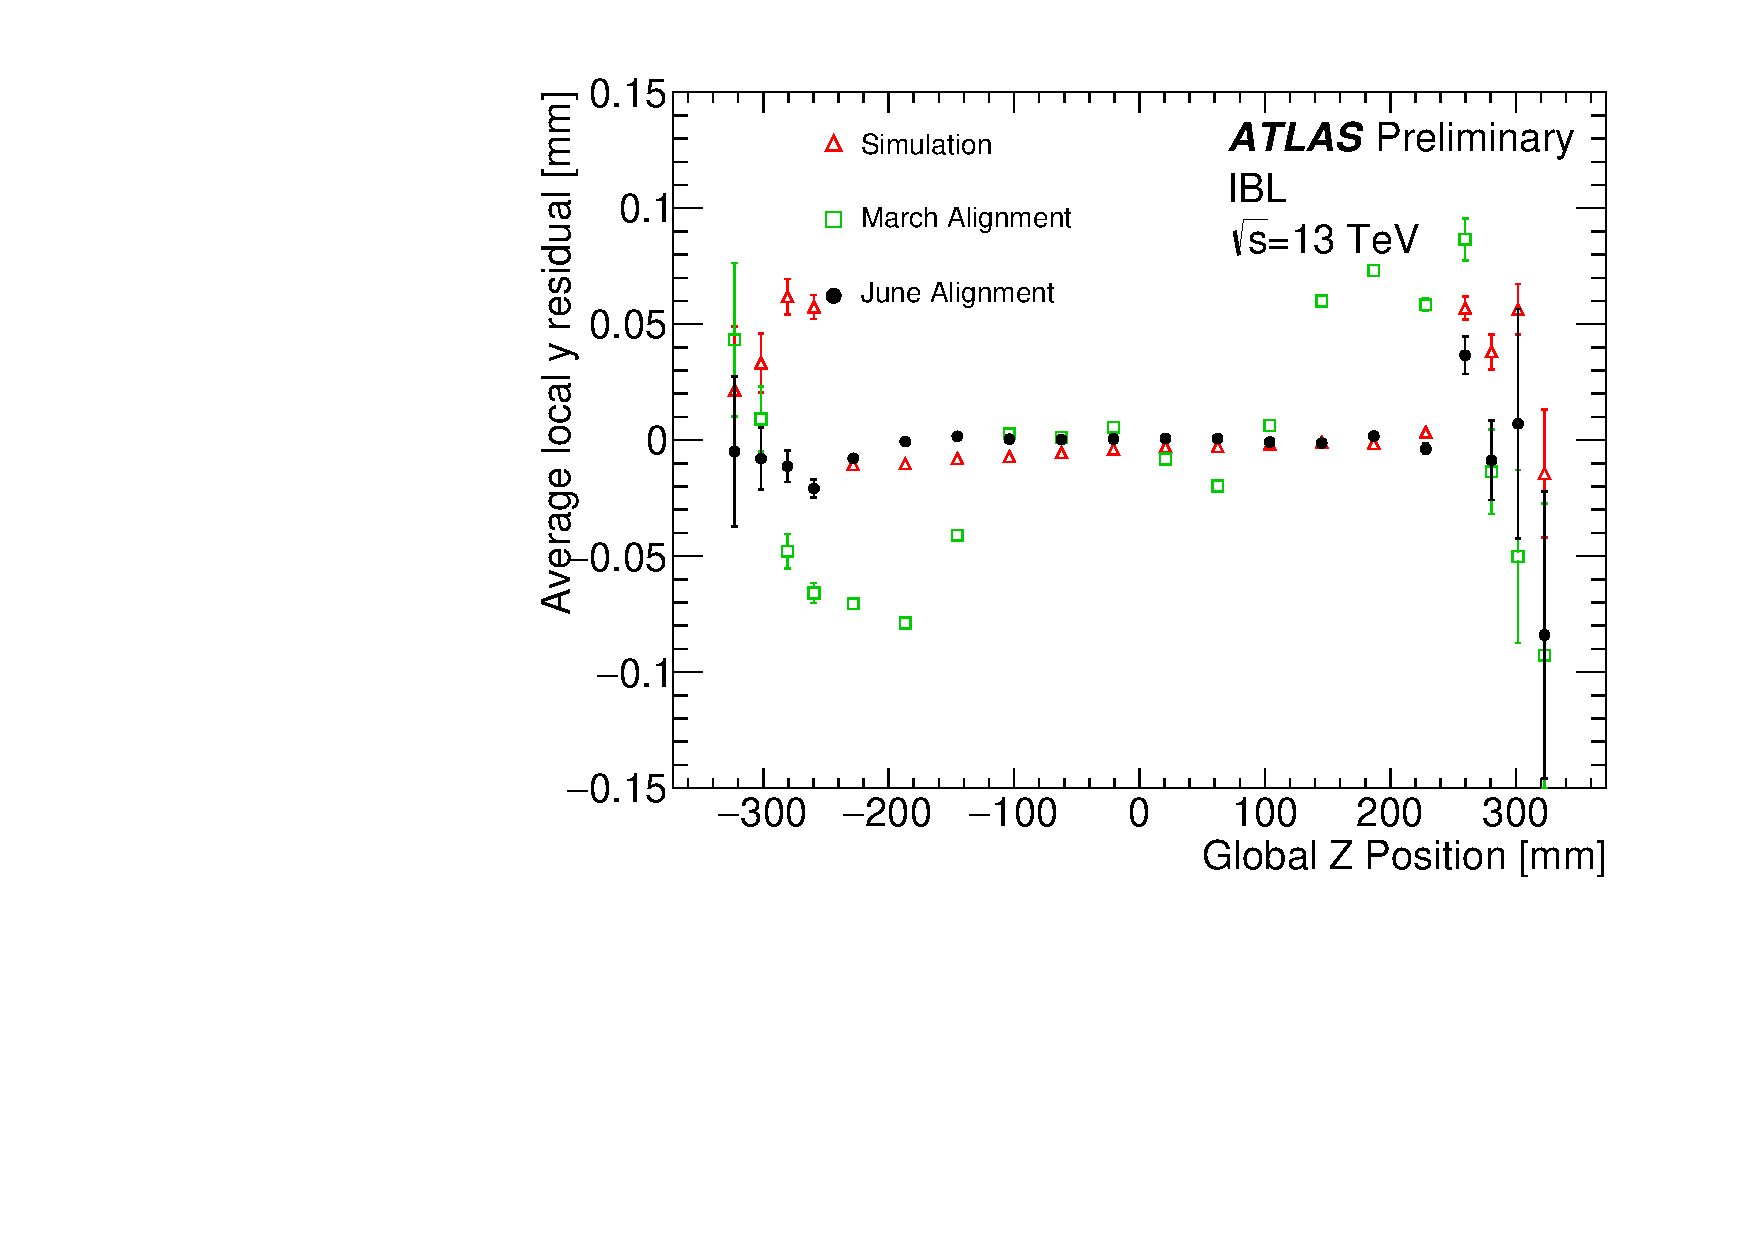
\includegraphics[width=.48\textwidth]{figs/alignment/align2015/IBL_yRESvsZ}
  \caption{The mean of the local $x$ (left) and local $y$ (right) residual distributions as a function of the global $z$ position of each IBL module using the \com{13} collision data sample reconstructed using the June (black) and March (green) alignments.  The data is compared to a MC simulation using a perfect detector geometry (red).}
  \label{fig:align_2015_results_ibl_z}.
\end{figure}

\begin{figure}[htbp]
  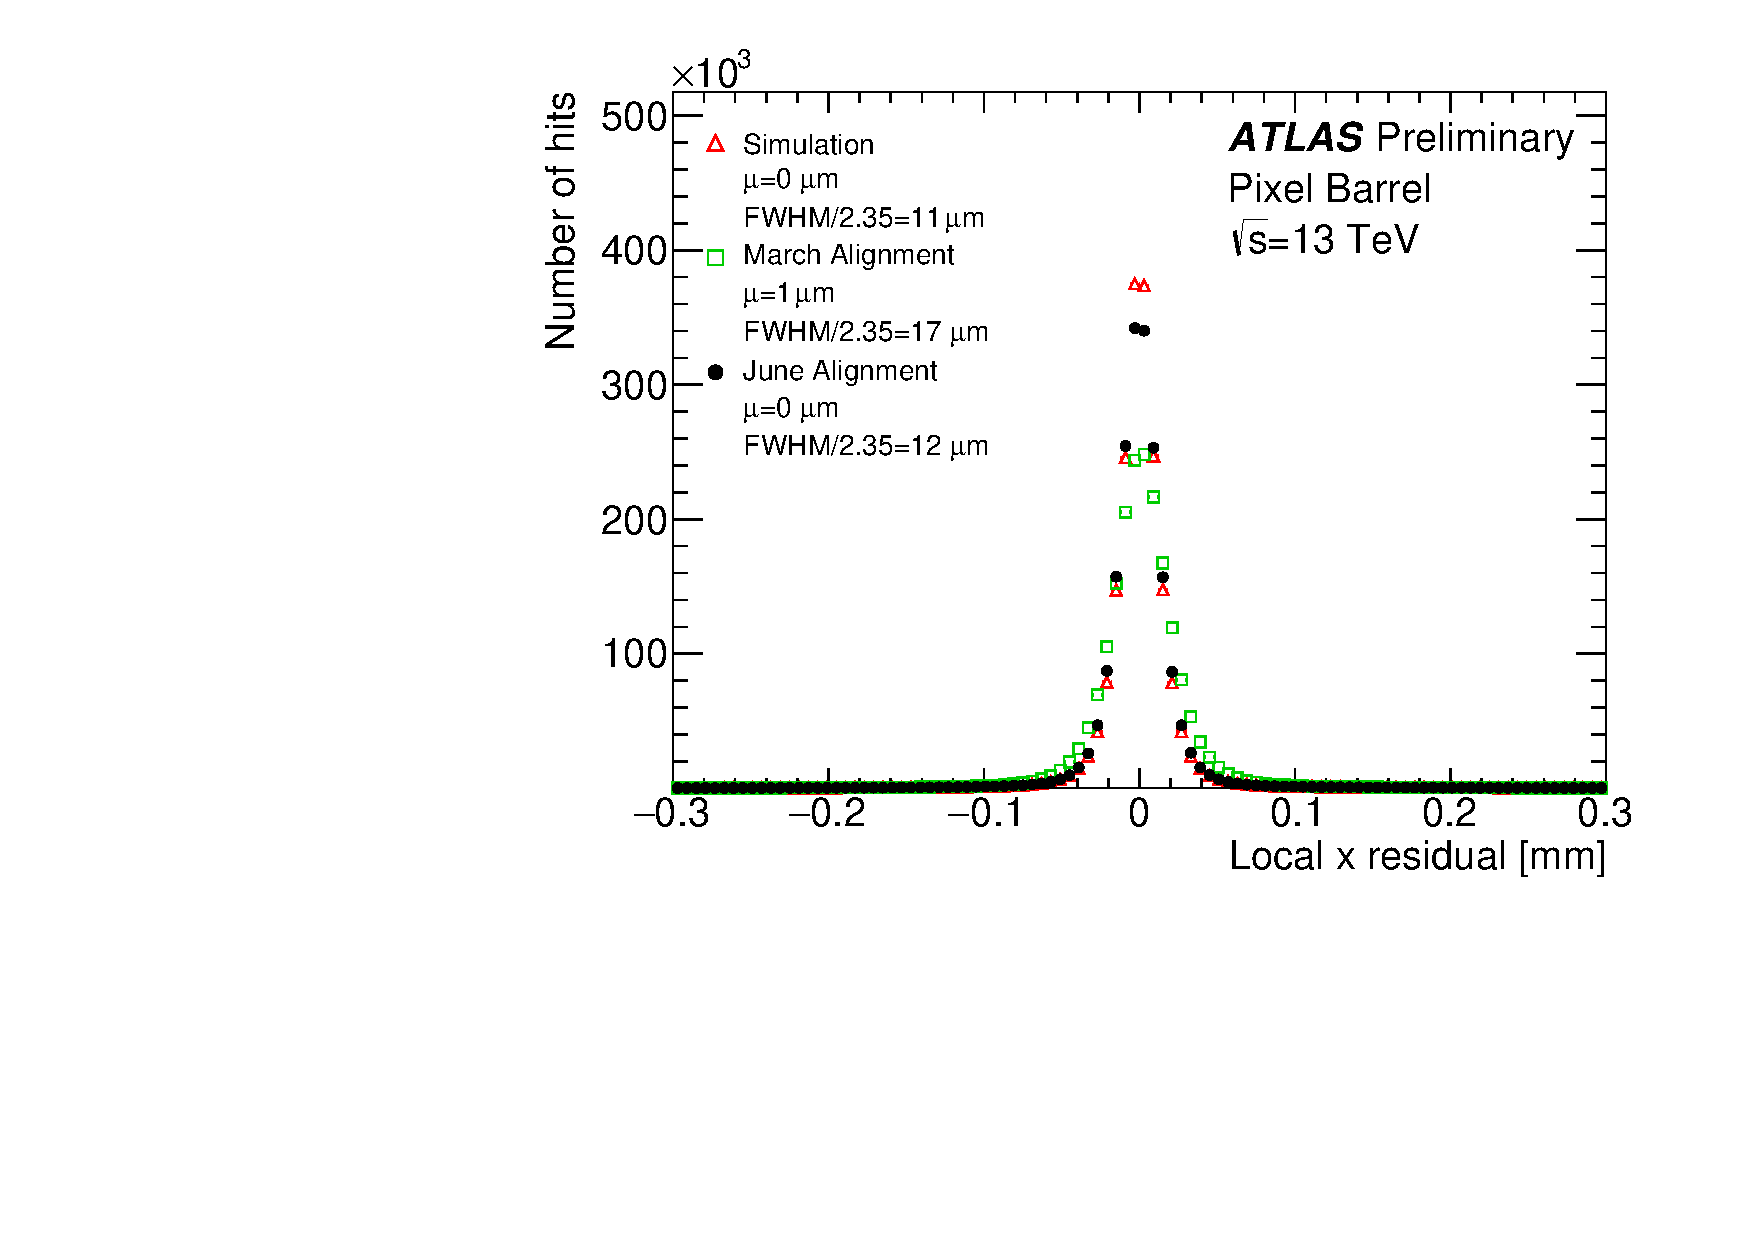
\includegraphics[width=.48\textwidth]{figs/alignment/align2015/OLDPIXX}
  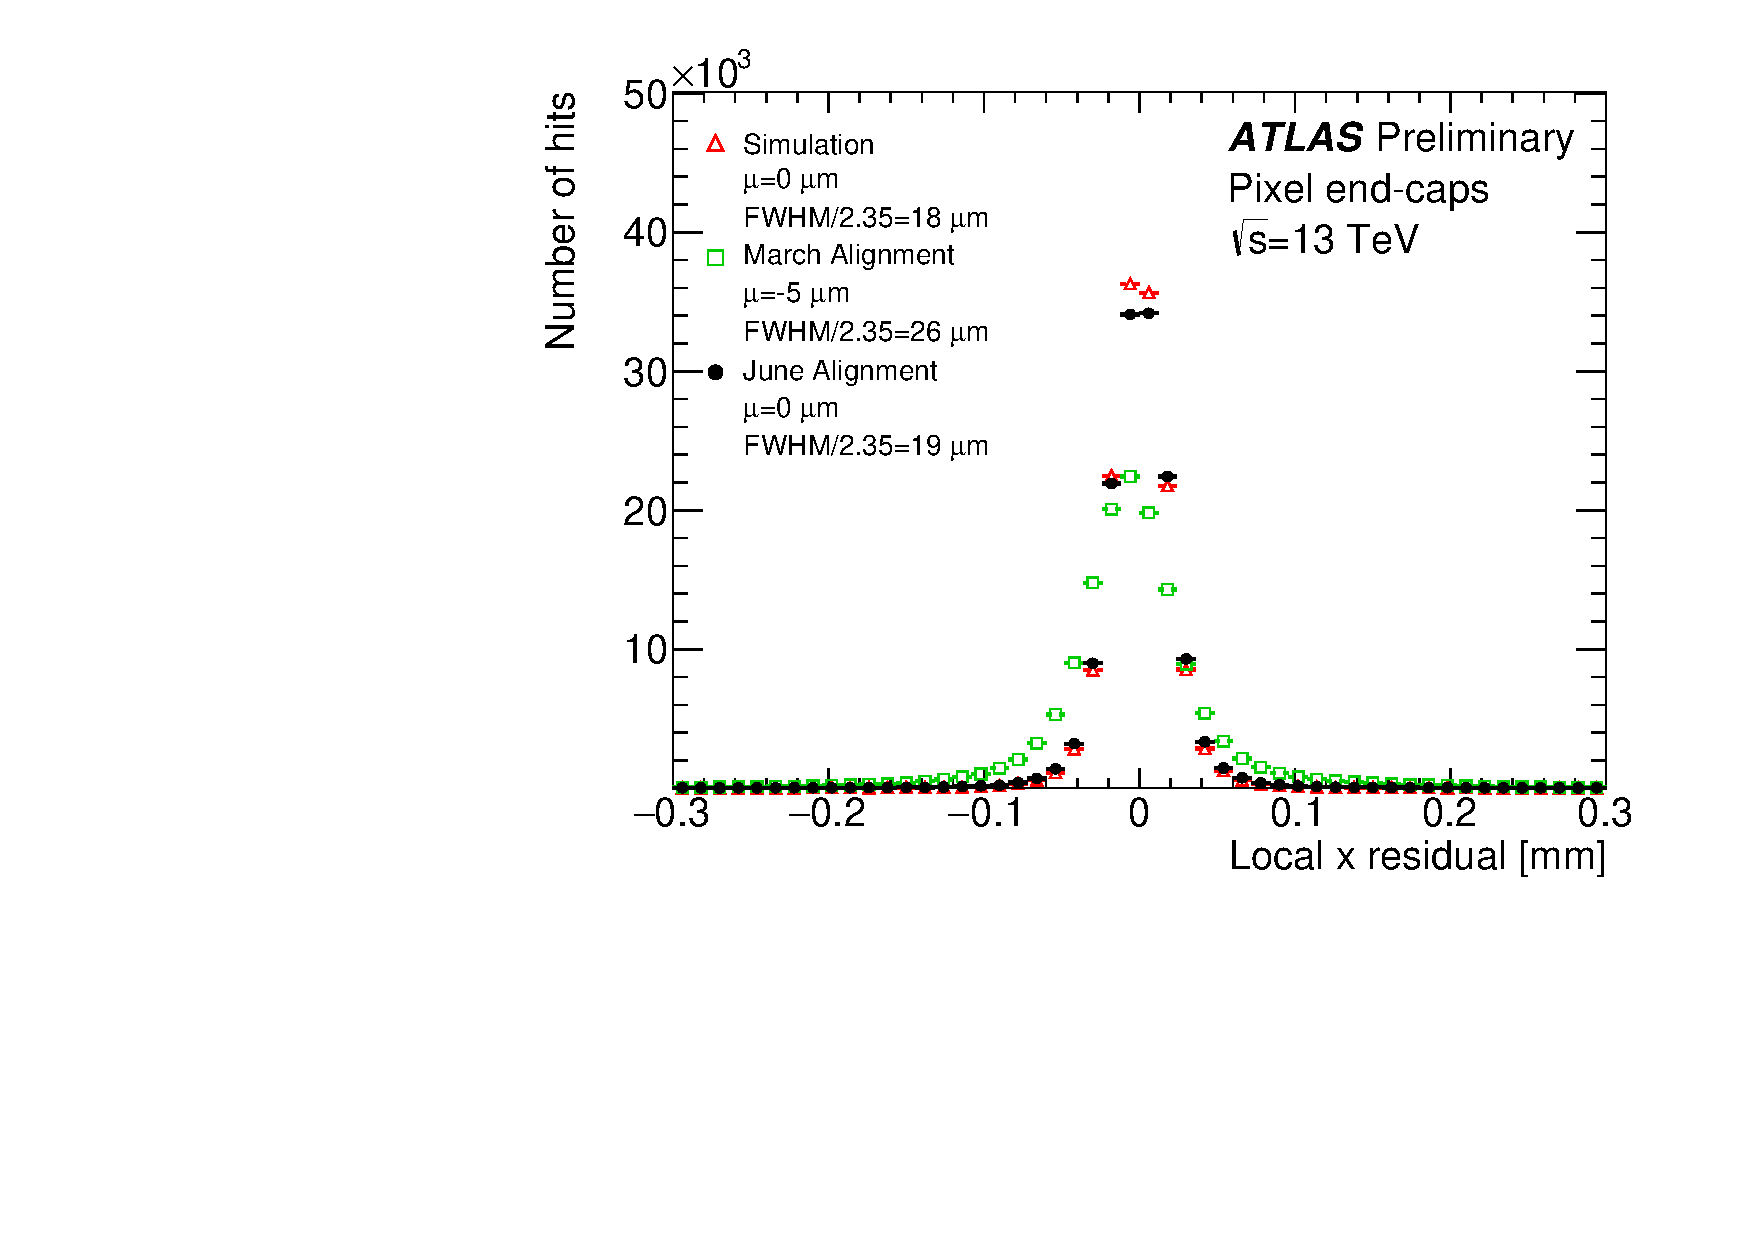
\includegraphics[width=.48\textwidth]{figs/alignment/align2015/PIXECX}\\
  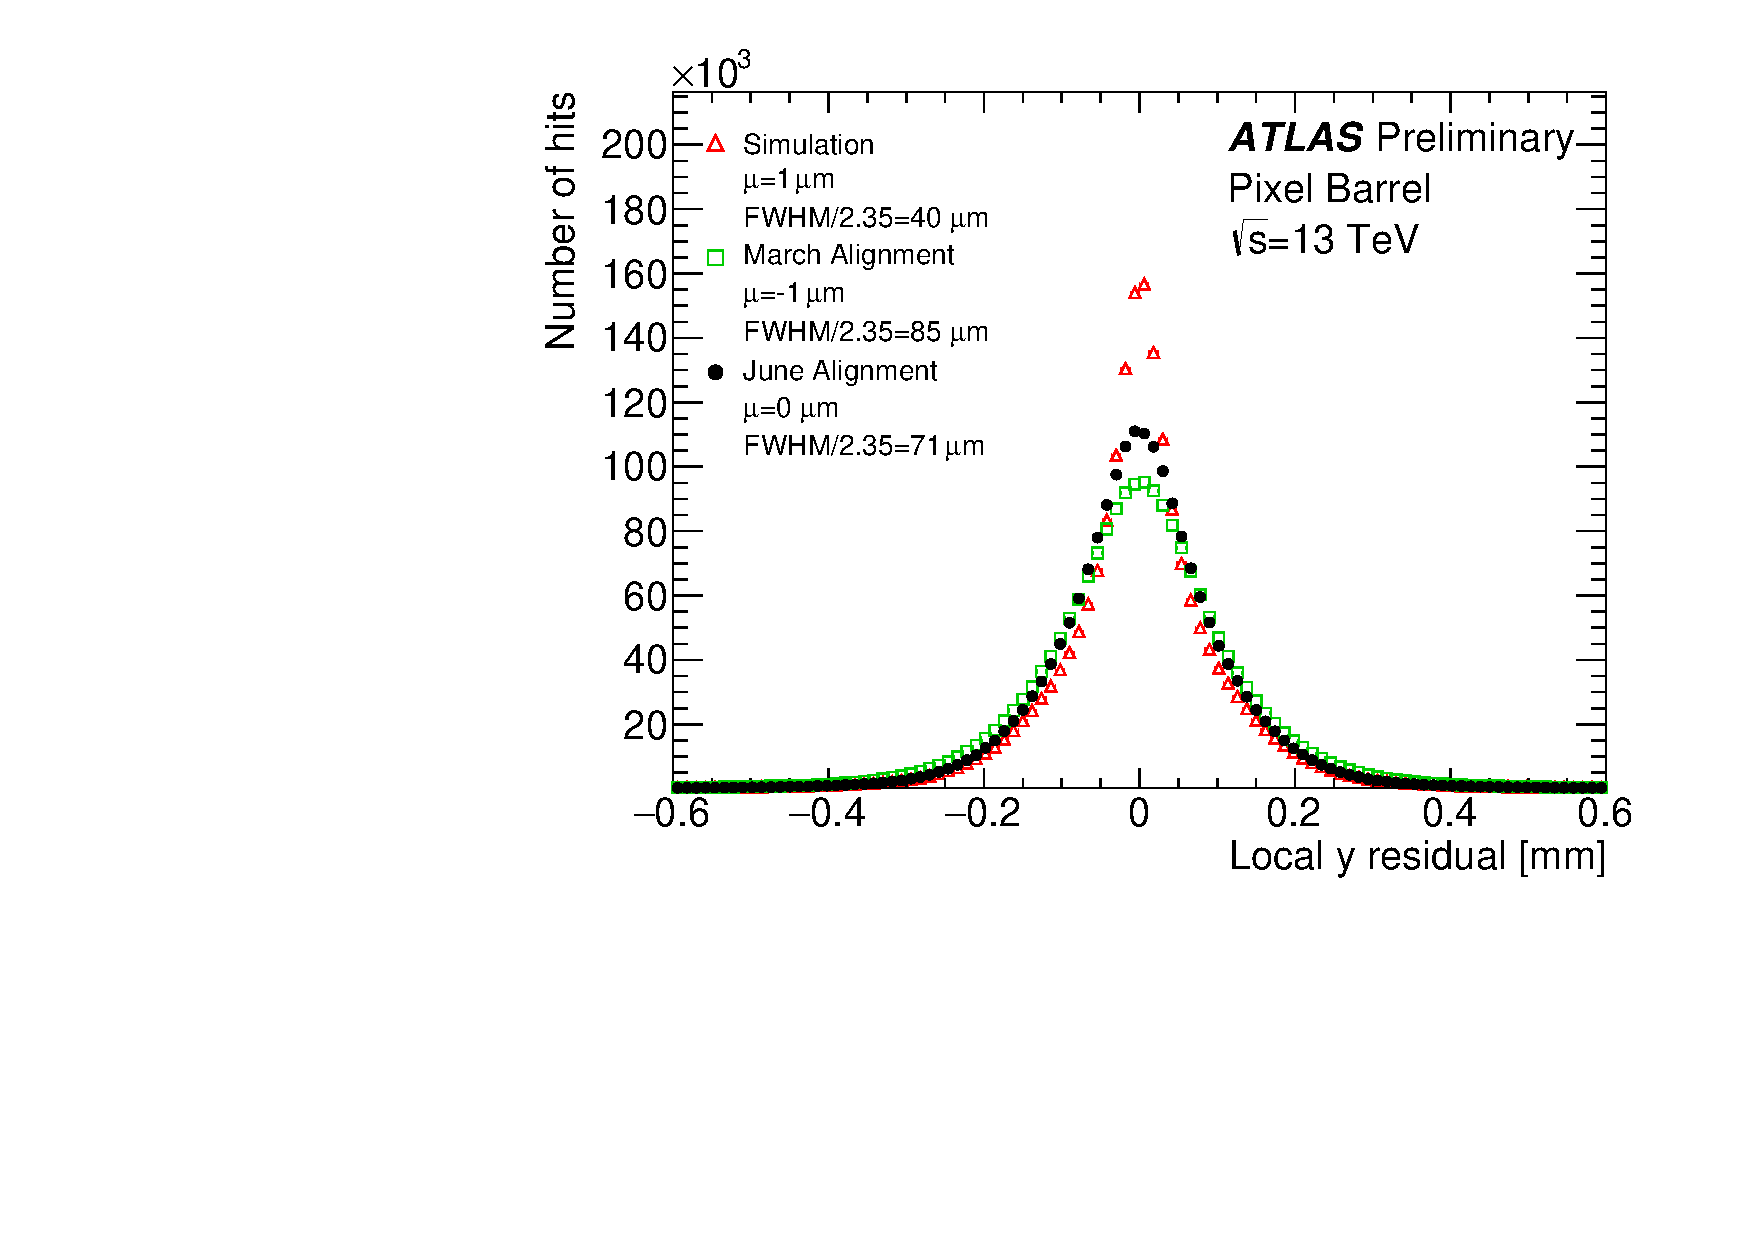
\includegraphics[width=.48\textwidth]{figs/alignment/align2015/OLDPIXY}
  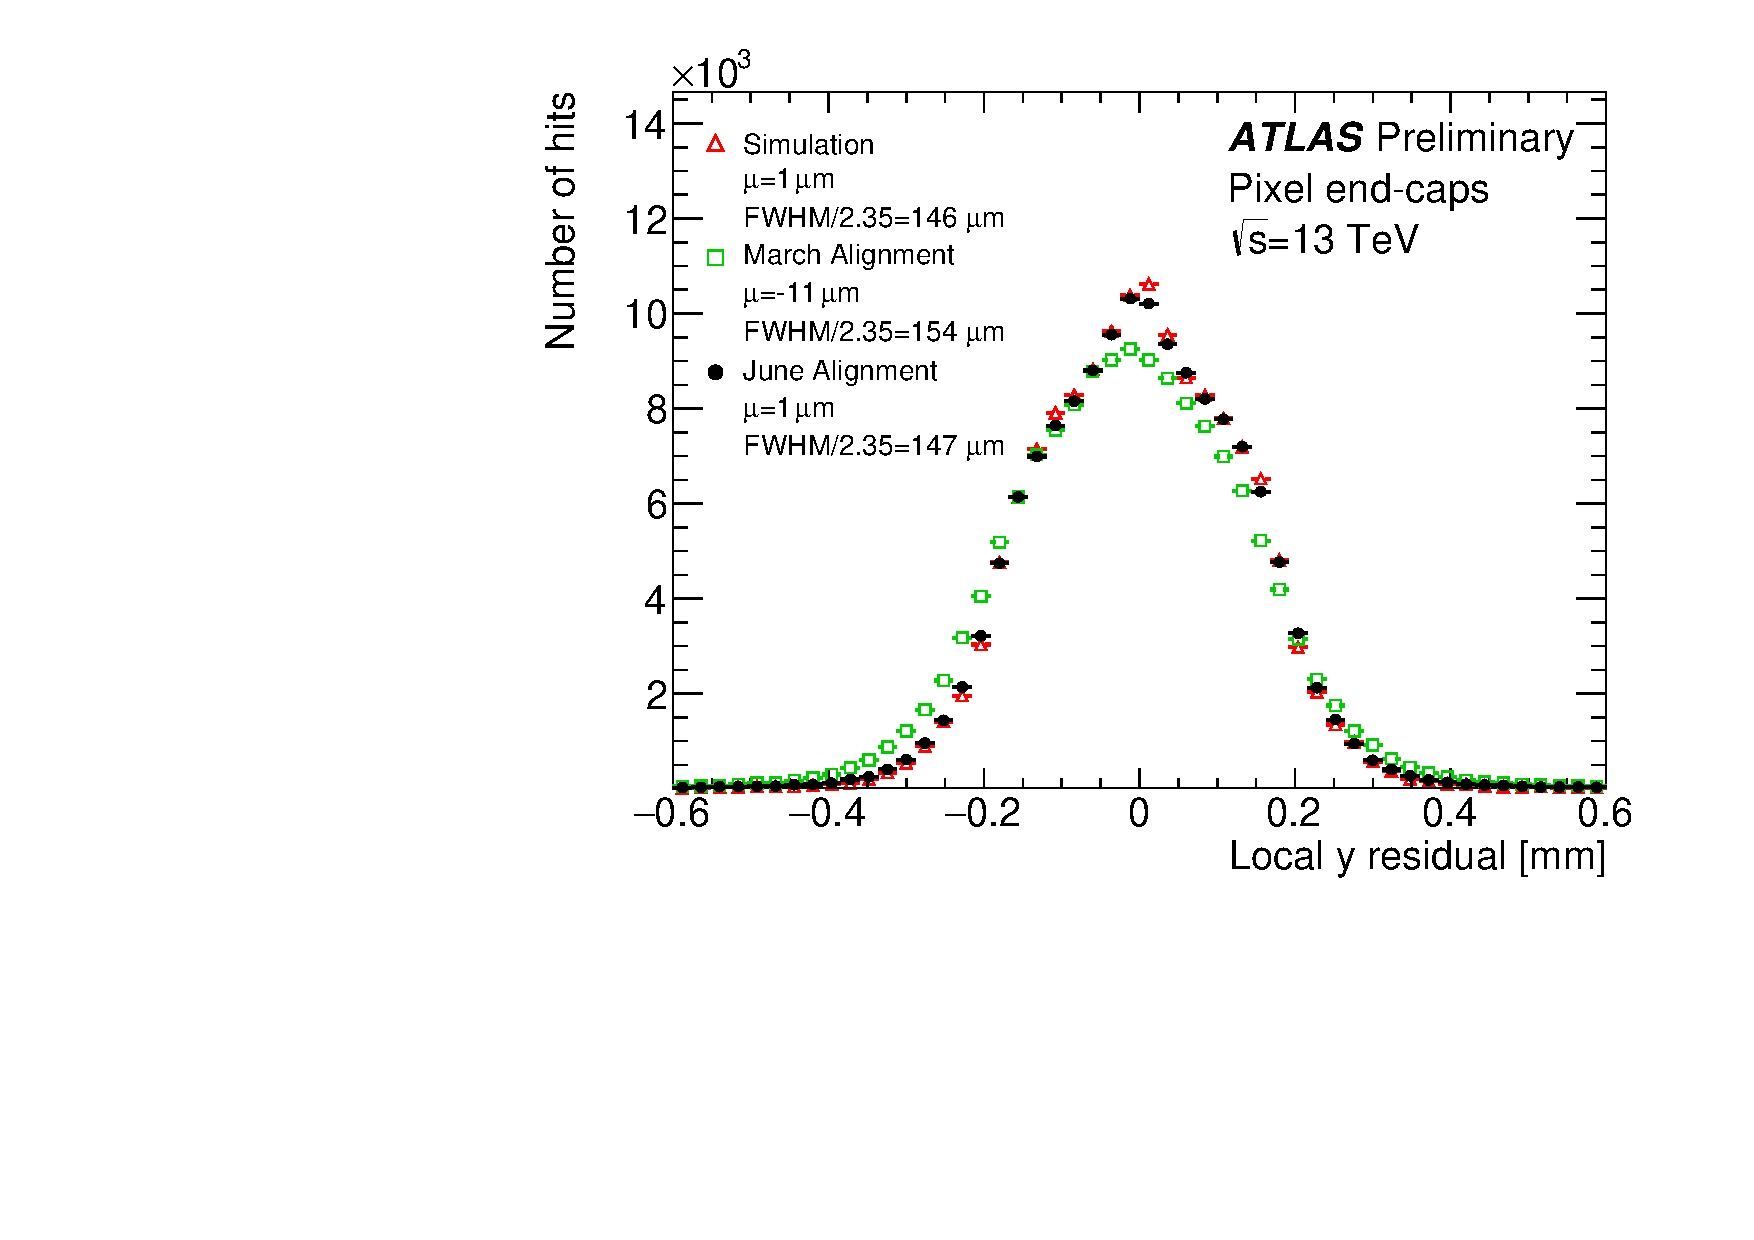
\includegraphics[width=.48\textwidth]{figs/alignment/align2015/PIXECY}
  \caption{Local $x$ (top) and local $y$ (bottom) residual distributions for the Pixel barrel (excluding the IBL, left) and end-caps (right) using the \com{13} collision data sample reconstructed using the June (black) and March (green) alignments.  The data is compared to a MC simulation using a perfect detector geometry (red).  The distributions are normalized to the same number of entries.}
  \label{fig:align_2015_results_pix}.
\end{figure}

Similar distributions for the SCT and TRT barrel and end-caps are shown in Figures~\ref{fig:align_2015_results_sct} and \ref{fig:align_2015_results_trt}, respectively.
Even though the TRT was not aligned at all, there is still some improvement in the width of the residuals between the March and June alignments due to the alignment of the other subdetectors improving the quality of the track fit.
The overall alignment of both these subdetectors despite neither being aligned at module-level indicates that the previous L3 alignment performed in Run 1 has not degraded significantly during the upgrade and maintenance period.

\begin{figure}[htbp]
  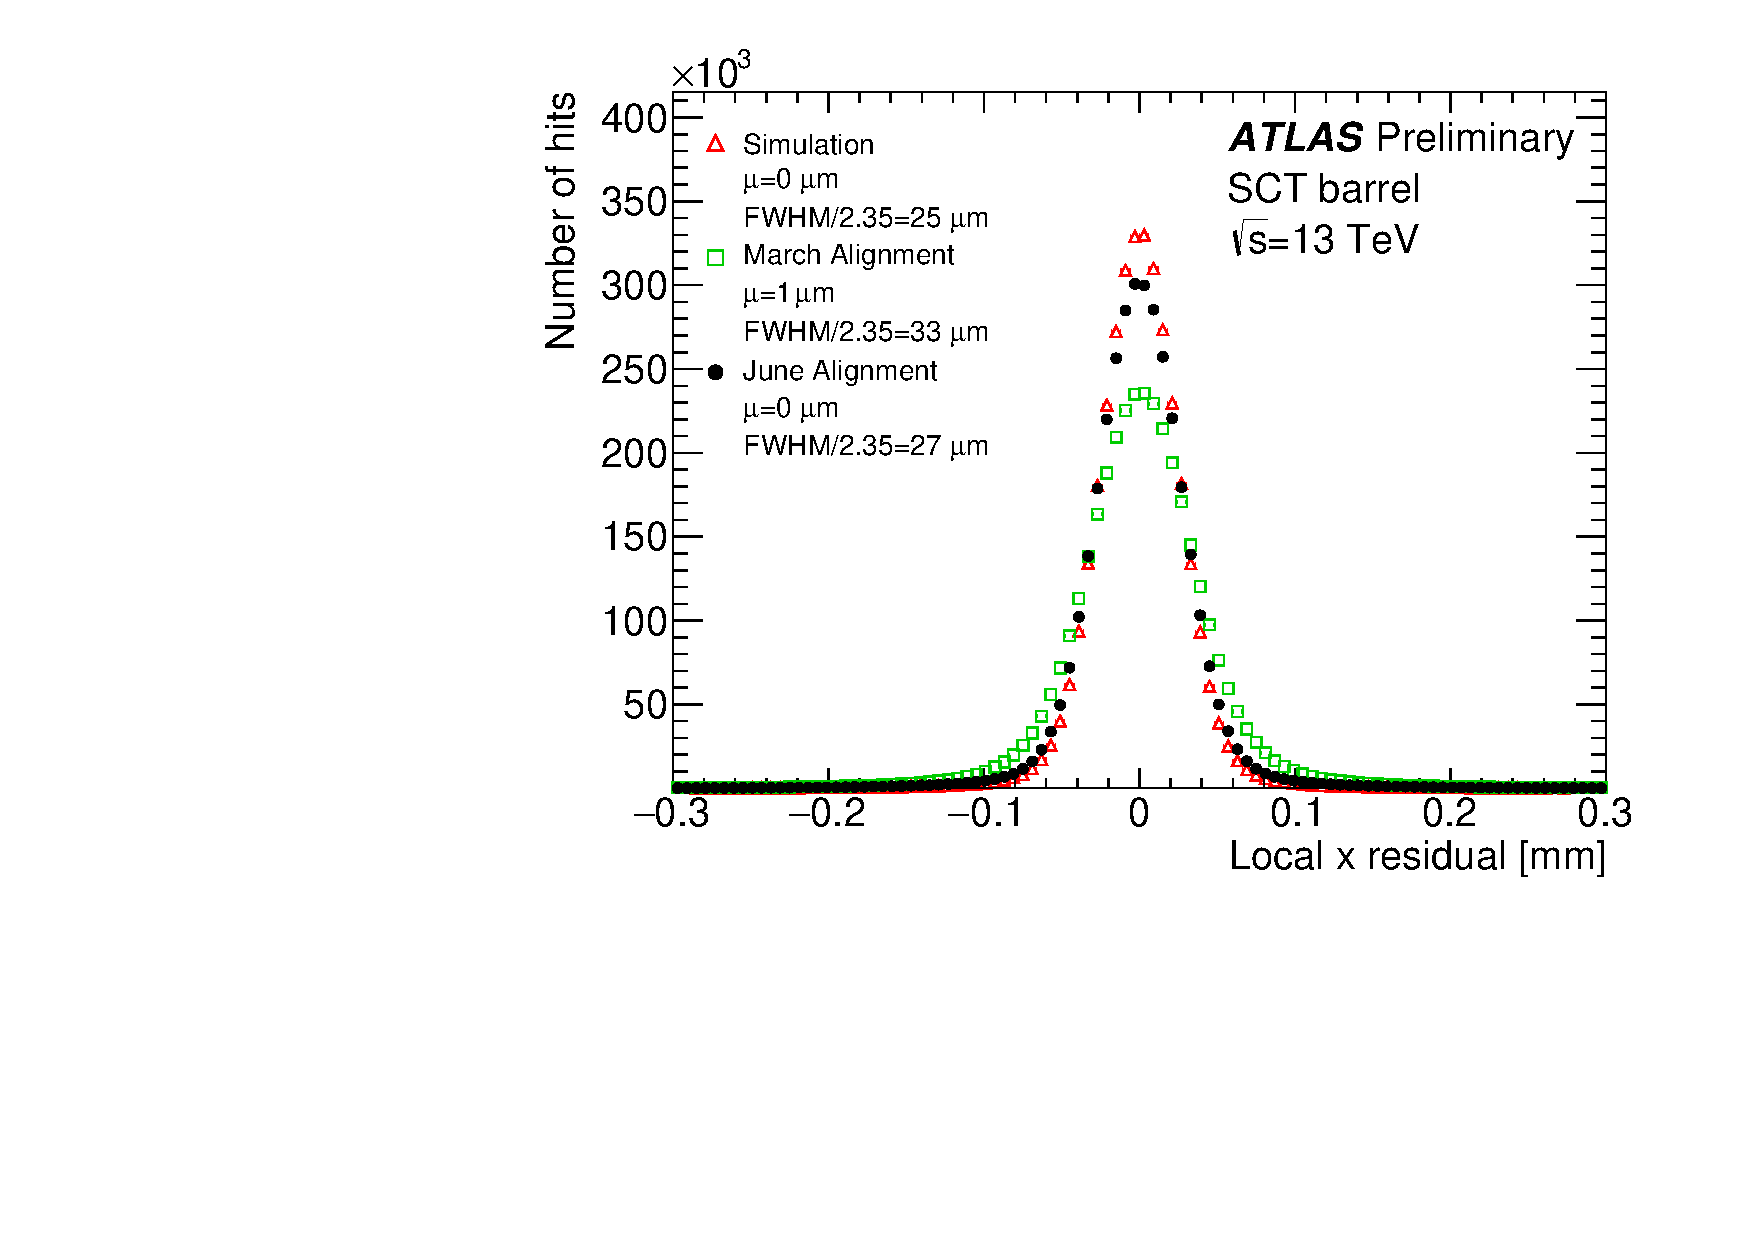
\includegraphics[width=.48\textwidth]{figs/alignment/align2015/SCTX}
  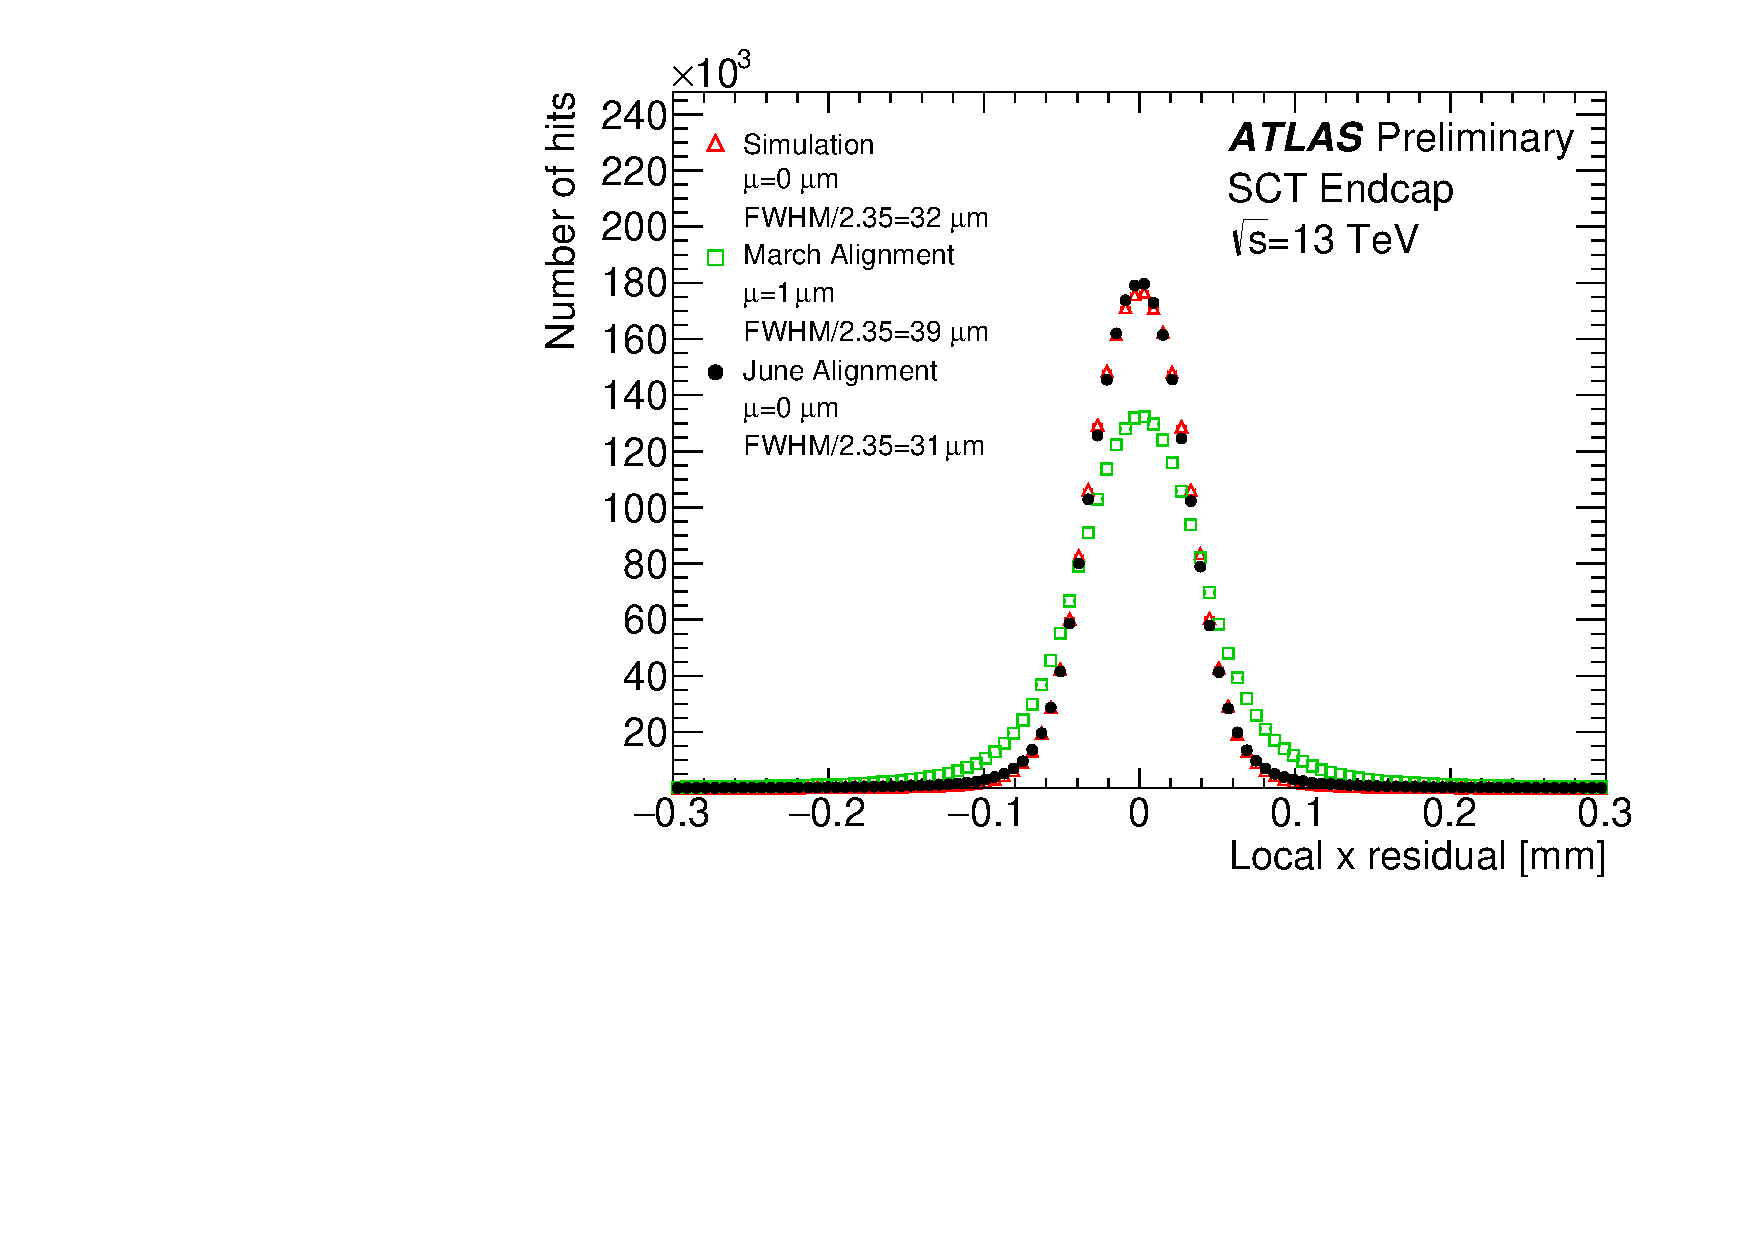
\includegraphics[width=.48\textwidth]{figs/alignment/align2015/SCTECX}
  \caption{Local $x$ residual distributions for the SCT barrel (left) and end-caps (right) using the \com{13} collision data sample reconstructed using the June (black) and March (green) alignments.  The data is compared to a MC simulation using a perfect detector geometry (red).  The distributions are normalized to the same number of entries.}
  \label{fig:align_2015_results_sct}.
\end{figure}

\begin{figure}[htbp]
  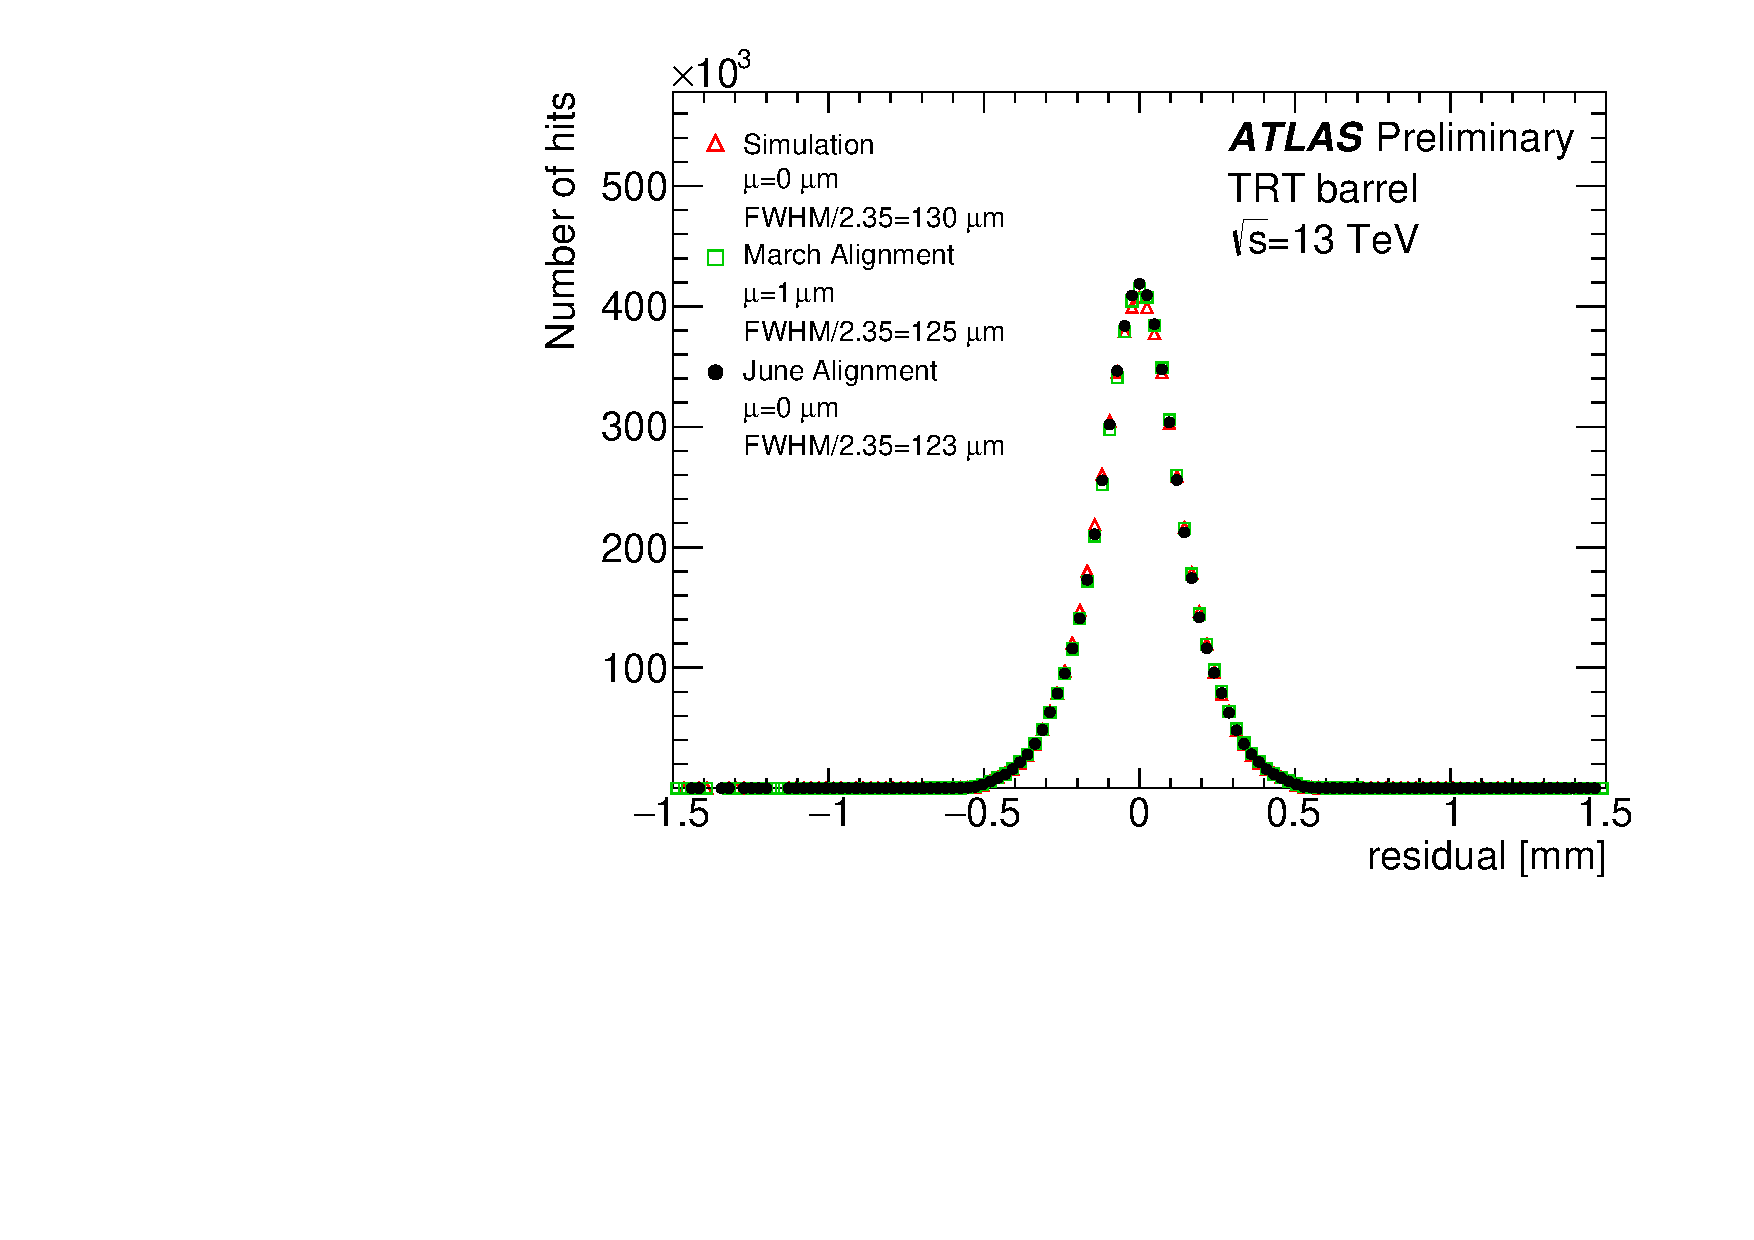
\includegraphics[width=.48\textwidth]{figs/alignment/align2015/TRTR}
  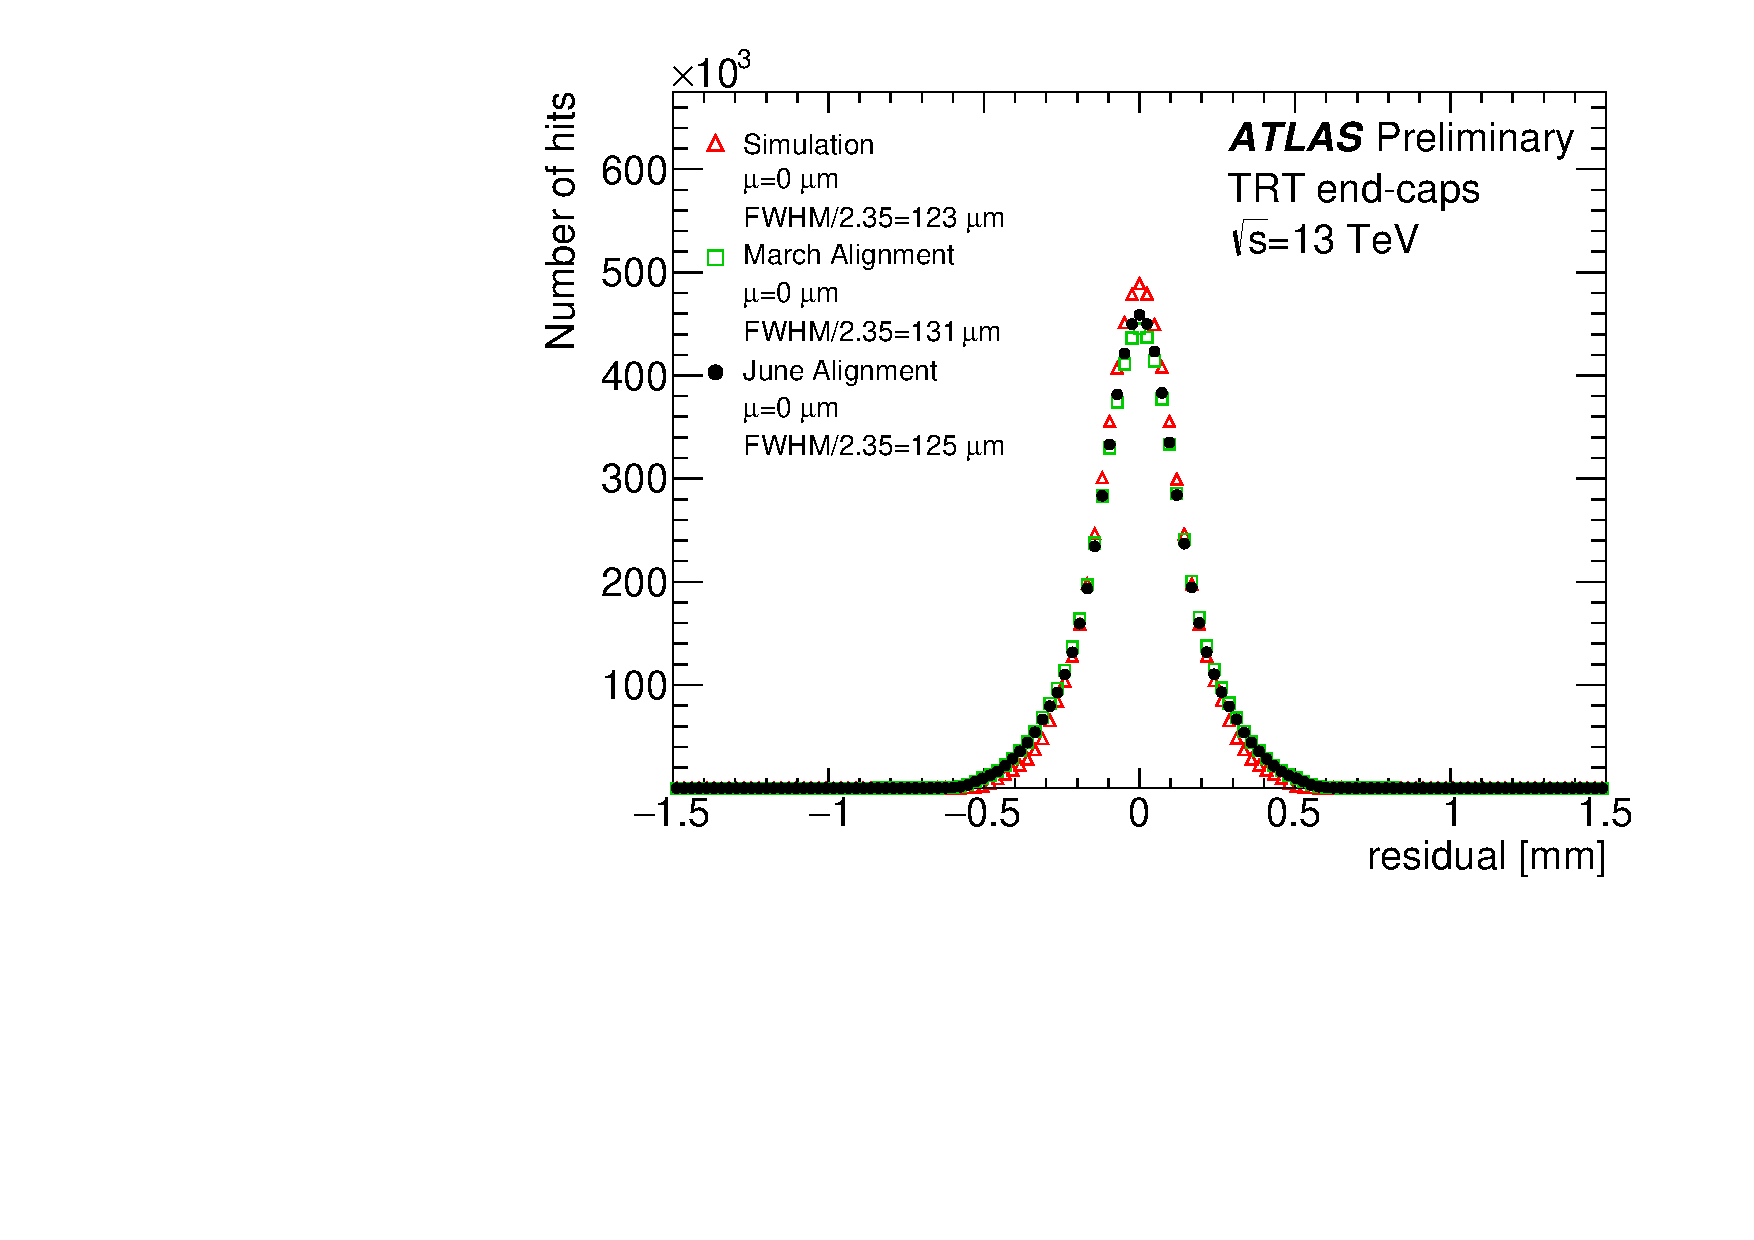
\includegraphics[width=.48\textwidth]{figs/alignment/align2015/TRTEC}
  \caption{Residual distributions for the TRT barrel (left) and end-caps (right) using the \com{13} collision data sample reconstructed using the June (black) and March (green) alignments.  The data is compared to a MC simulation using a perfect detector geometry (red).  The distributions are normalized to the same number of entries.}
  \label{fig:align_2015_results_trt}.
\end{figure}

\subsubsection{Track parameter resolution from cosmic rays}\label{align:2015_results_cosmic}

%\section{Additional alignment efforts}
%\subsection{L2 alignment of the TRT}
%\subsection{Alignment of the IBL}\label{align:ibl}
%thinking this should probably be a section not a subsection since it's not directly related to the 2015 paper i'm basing the previous section on... idk.
